\documentclass{beamer}
%
% Choose how your presentation looks.
%
% For more themes, color themes and font themes, see:
% http://deic.uab.es/~iblanes/beamer_gallery/index_by_theme.html
%
\mode<presentation>
{
  \usetheme{default}      % or try Darmstadt, Madrid, Warsaw, ...
  \usecolortheme{default} % or try albatross, beaver, crane, ...
  \usefonttheme{default}  % or try serif, structurebold, ...
  \setbeamertemplate{navigation symbols}{}
  \setbeamertemplate{caption}[numbered]
} 

\usepackage[english]{babel}
\usepackage[utf8x]{inputenc}

\title[Spectral Graph Theory Applications]{Control architectures for co-operative control of mobile robots}
\author{Adwait Datar}
\institute{PhD Workshop, 2020\\Technical University of Hamburg}
\date{$16^{th}$ Oct,2020}

\begin{document}

\begin{frame}	
  \titlepage
\end{frame}

% Uncomment these lines for an automatically generated outline.
%\begin{frame}{Outline}
%  \tableofcontents
%\end{frame}
%%%%%%%%%%%%%%%%%%%%%%%%%%%%%%%%%%%%%%%%%%%%%%%%%%%%%%%%%%%%%%%%%%%%%
\begin{frame}{Motivating Scenarios}
	Fukushima Disaster (2011)
	%\footnote{https://rememberfukushima.org/fallout-maps/}
	\hspace{0.4 cm}
	Truck Platoon Competition (2016)
	%\footnote{https://response.restoration.noaa.gov}
	\\
	\begin{minipage}{0.45\textwidth}	
		\begin{figure}
			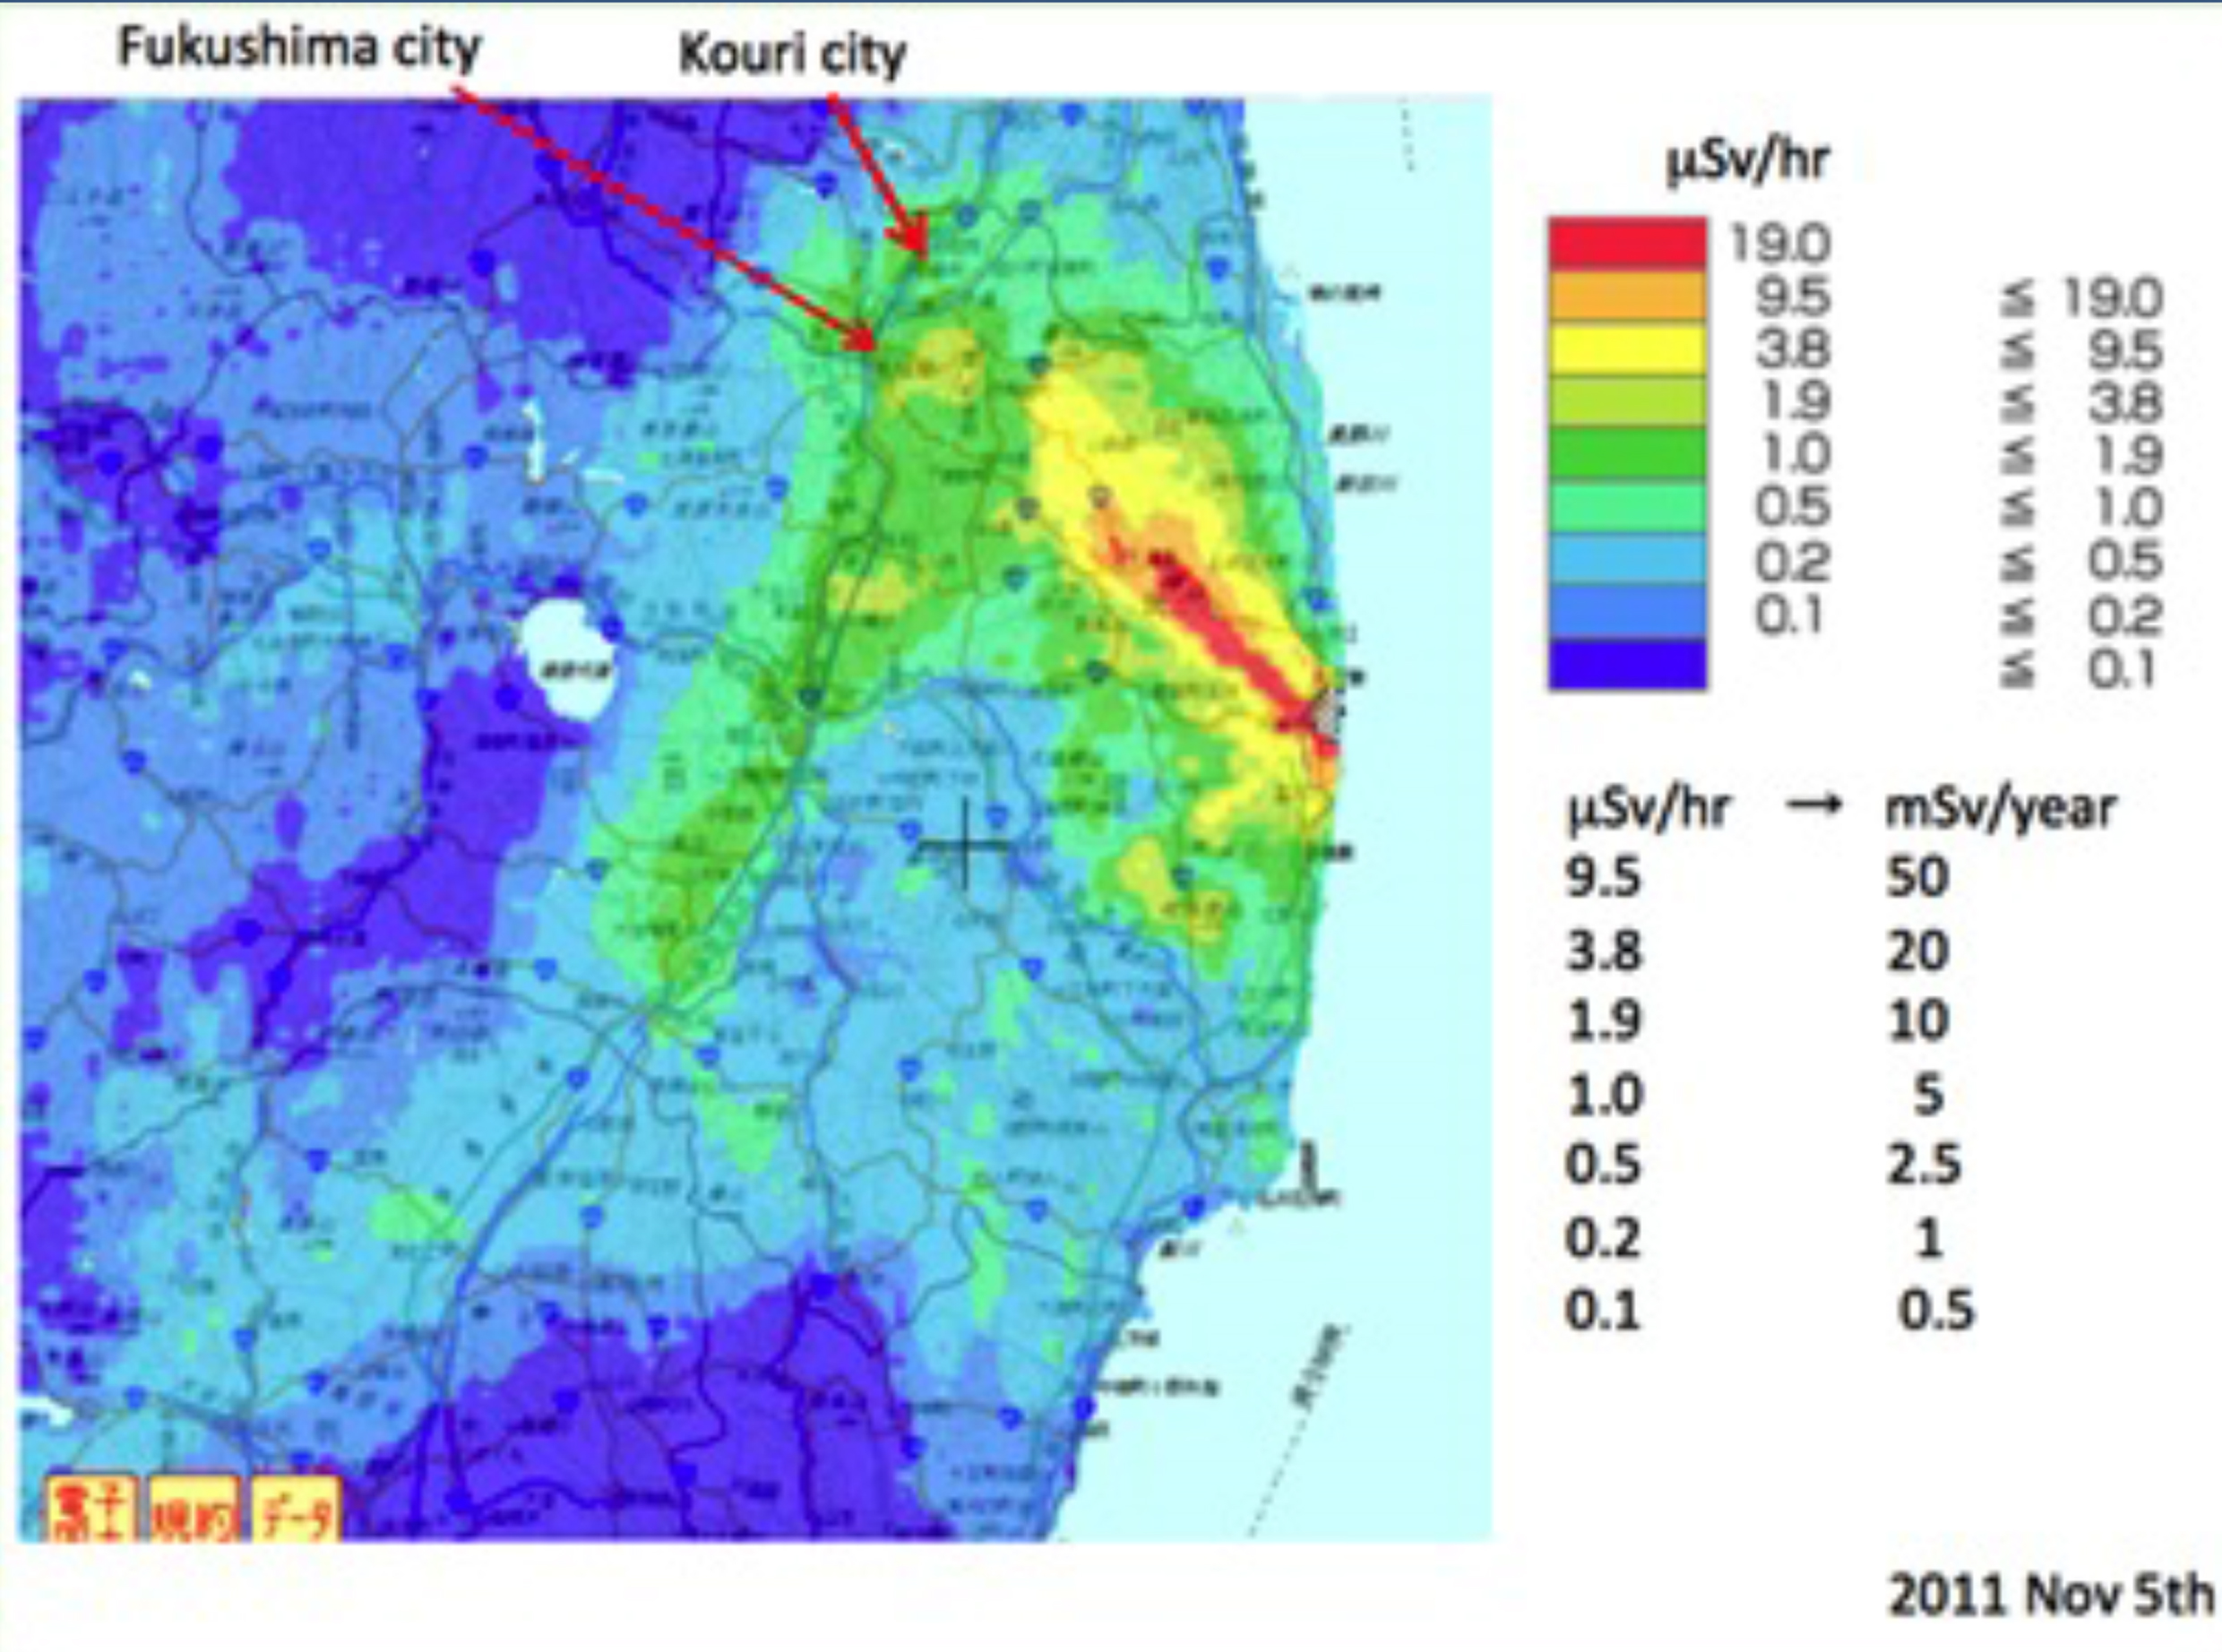
\includegraphics[width=1\textwidth]{figures/fukushima_disaster.jpg}
			%\caption{Fukushima Disaster (2011)}
			%\label{fig:fukushima_disaster}
		\end{figure}
		\begin{figure}
			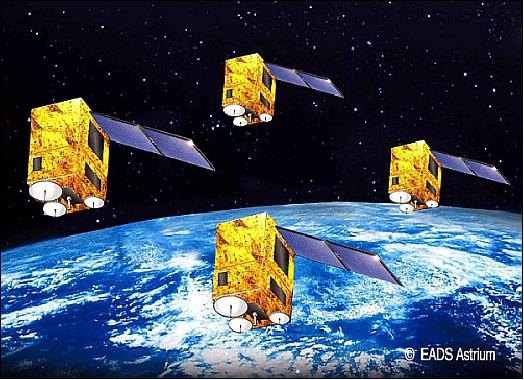
\includegraphics[scale=0.2]{figures/Essaim_constellation.jpg}\label{fig:satellite_flock}
		\end{figure}
	\end{minipage}
	\hspace{0.05cm}
	\begin{minipage}{0.45\textwidth}
		\begin{figure}
			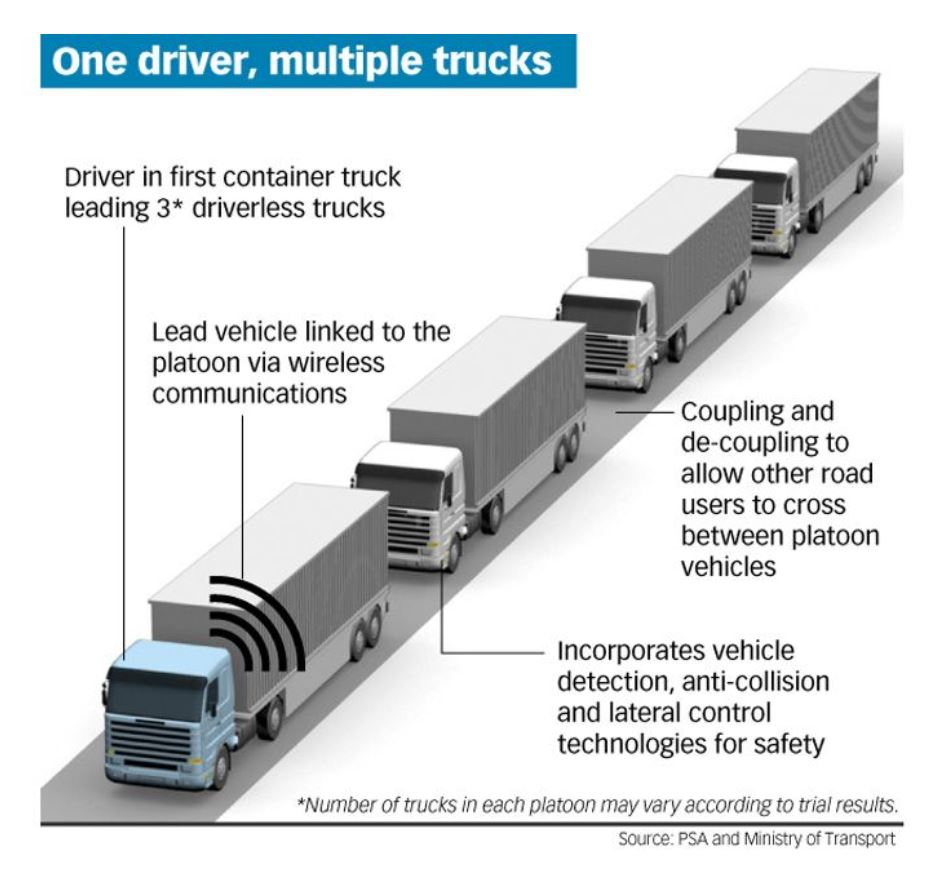
\includegraphics[height=0.4\textheight]{figures/truck_platoon.jpg}
			%\caption{Oil Spills}
			%\label{fig:oilspills}
		\end{figure}
		\begin{figure}
			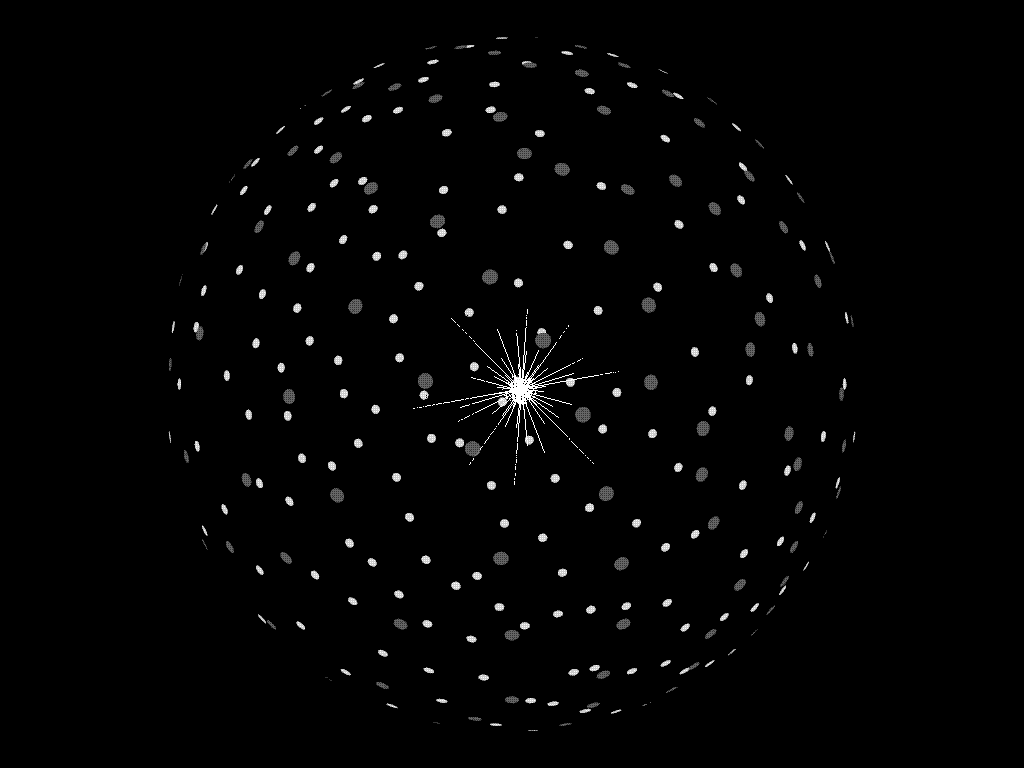
\includegraphics[scale=0.1]{figures/Dyson_swarm.png}		
			\label{fig:Dyson_swarms}
		\end{figure}	
	\end{minipage}
	
	.
	\hspace{0.5 cm}
	EADS Astrium 
	%\footnote{https://earth.esa.int}
	\hspace{1.7 cm}
	Dyson Swarm (Why not !)
	\\
	%\vspace{0.5cm}
	%\begin{itemize}
	%	\item Disaster striken areas could be dangerous and potentially life threatening for humans 
	%	\item Deploy a swarm of autonomous robots with sensing and communication capabilities to locate the source of accident.
	%\end{itemize}
\end{frame}
%%%%%%%%%%%%%%%%%%%%%%%%%%%%%%%%%%%%%%%%%%%%%%%%%%%%%%%%%%%%%%%%%%%%%
\begin{frame}{Abstracting to a Mathematical Problem}	
\begin{block}{Problem Statement:}
Design distributed control algorithms for large networks of mobile robots such that the group shows a desirable behavior.
\end{block}
\begin{itemize}
	\item Desirable behaviors we consider:
	\begin{itemize}
		\item Consensus and/or Formation stabilization
		\item Flocking with/without source seeking
	\end{itemize}	
	\item Complexity in solving the problem can stem through:
	\begin{itemize}
		\item Complicated dynamics of individual agents
		\item Commplicated Interconnection structure and intractible design algorithms for large networks
	\end{itemize}
\end{itemize}
\end{frame}
%%%%%%%%%%%%%%%%%%%%%%%%%%%%%%%%%%%%%%%%%%%%%%%%%%%%%%%%%%%%%%%%%%%%%
\begin{frame}{Approaching the problem: Divide and Conquer}
\begin{block}{Available literature on}
\begin{itemize}
	\item Control of single complex agent dynamics (e.g LPV, control of differetially flat systems, dynamic inversion) 
	\item Distributed control of large networks of "simple" agent dynamics (e.g single and double intergrators) -> Consensus and Flocking algorithms
\end{itemize}
\end{block}	
\begin{block}{Consider as building blocks}
\begin{itemize}
	\item Closed-loop system $G_{\textnormal{cl}}$ with some guaranteed performance measure such as the induced $\mathcal{L}_2-\mathcal{L}_2$ or  $\mathcal{L}_2-\mathcal{L}_{\infty}$ norms
	\item Consensus or Flocking algorithms for "simple" systems
\end{itemize}
\end{block}
\end{frame}
%%%%%%%%%%%%%%%%%%%%%%%%%%%%%%%%%%%%%%%%%%%%%%%%%%%%%%%%%%%%%%%%%%%%%
\begin{frame}{Consensus/ Formation with a decoupled architecture: \\"Small" disturbances and "good" tracking}
\begin{figure}
	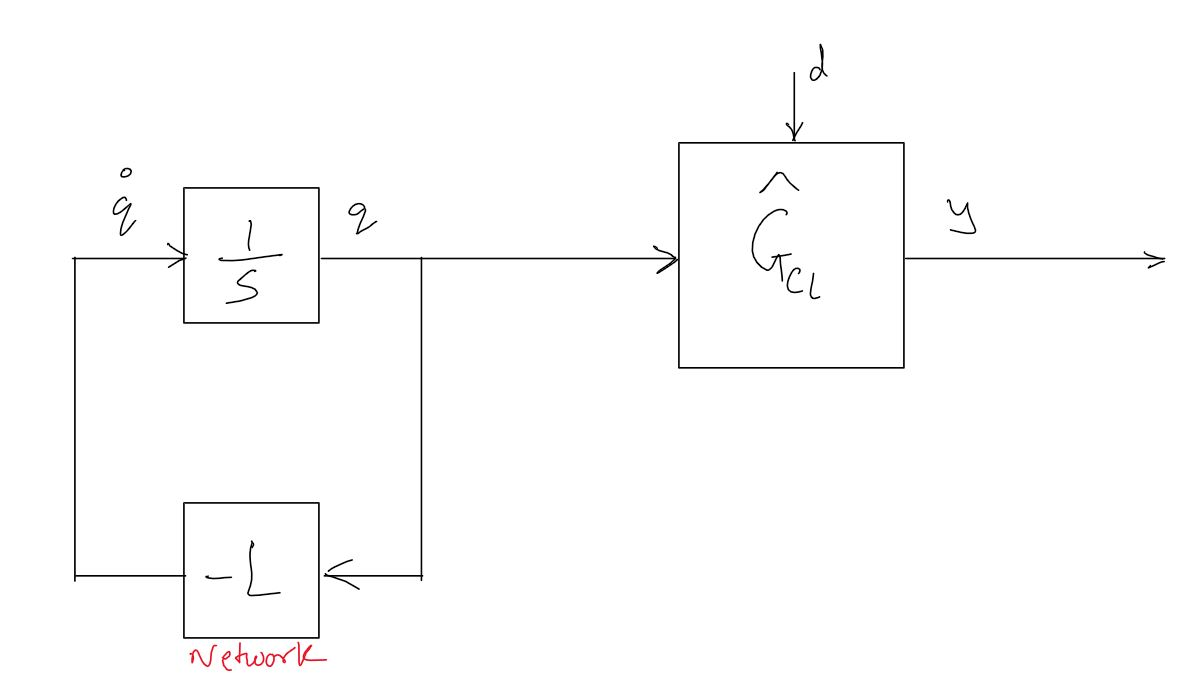
\includegraphics[height=0.45\textheight]{figures/cons_decoupled.jpg}
	%\caption{Oil Spills}
	%\label{fig:oilspills}
\end{figure}
\begin{itemize}
	\item Can bound the $||q-y||_{\mathcal{L}_{\infty}}$ to get an idea about how far the true trajectories given a bound on the disturbance
	\item C. Hespe, A. Datar, and H. Werner, “Distributed control of mobile lti and lpv agents using induced $\mathcal{L}_2$ to $\mathcal{L}_{\infty}$ norms.”
	\item Discrete-time, positive systems theory-> ACC Submission
\end{itemize}
\end{frame}
%%%%%%%%%%%%%%%%%%%%%%%%%%%%%%%%%%%%%%%%%%%%%%%%%%%%%%%%%%%%%%%%%%%%%
\begin{frame}{Flocking with a decoupled architecture:\\ "slow" flocking and "good" tracking}
	\begin{figure}
		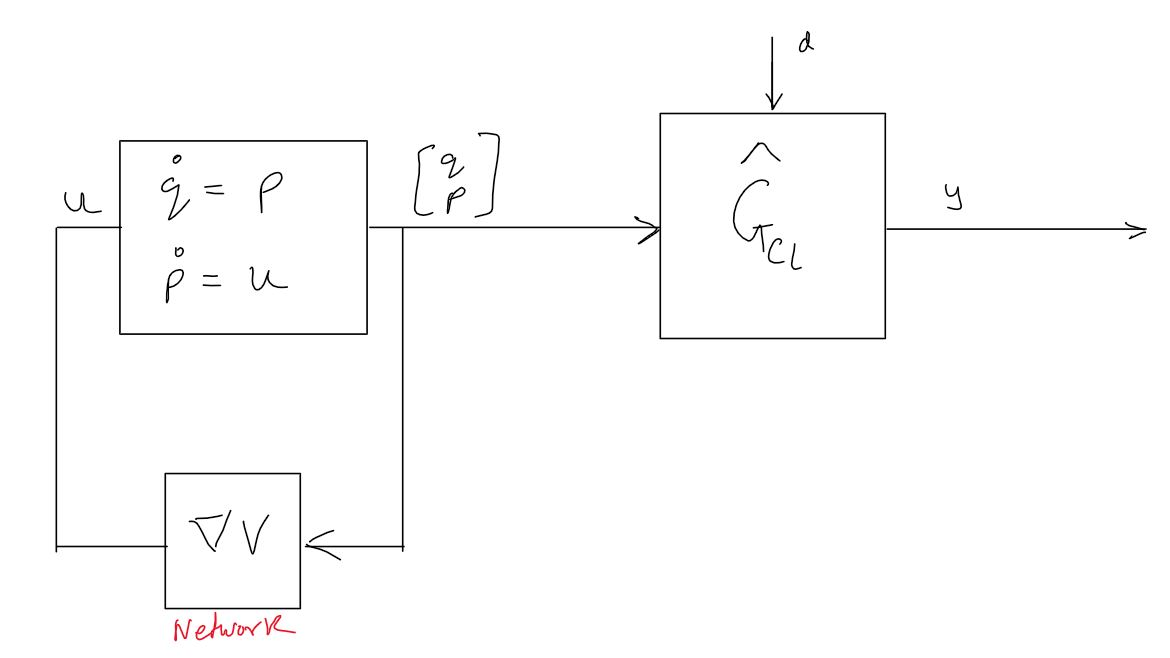
\includegraphics[height=0.45\textheight]{figures/Flocking_decoupled.jpg}
		%\caption{Oil Spills}
		%\label{fig:oilspills}
	\end{figure}
	\begin{itemize}		
		\item Experimental work: Datar, Adwait, Paulsen, Peter and Werner, Herbert (2020): Flocking Towards the Source: Indoor Experiments with Quadrotors. In 2020 European Control Conference (ECC) (pp. 1638-1643).
		\item Local Velocity Controller
		\item \textcolor{red}{No Analysis yet}
	\end{itemize}
\end{frame}
%%%%%%%%%%%%%%%%%%%%%%%%%%%%%%%%%%%%%%%%%%%%%%%%%%%%%%%%%%%%%%%%%%%%%
\begin{frame}{Consensus with a Coupled architecture}
\begin{figure}
	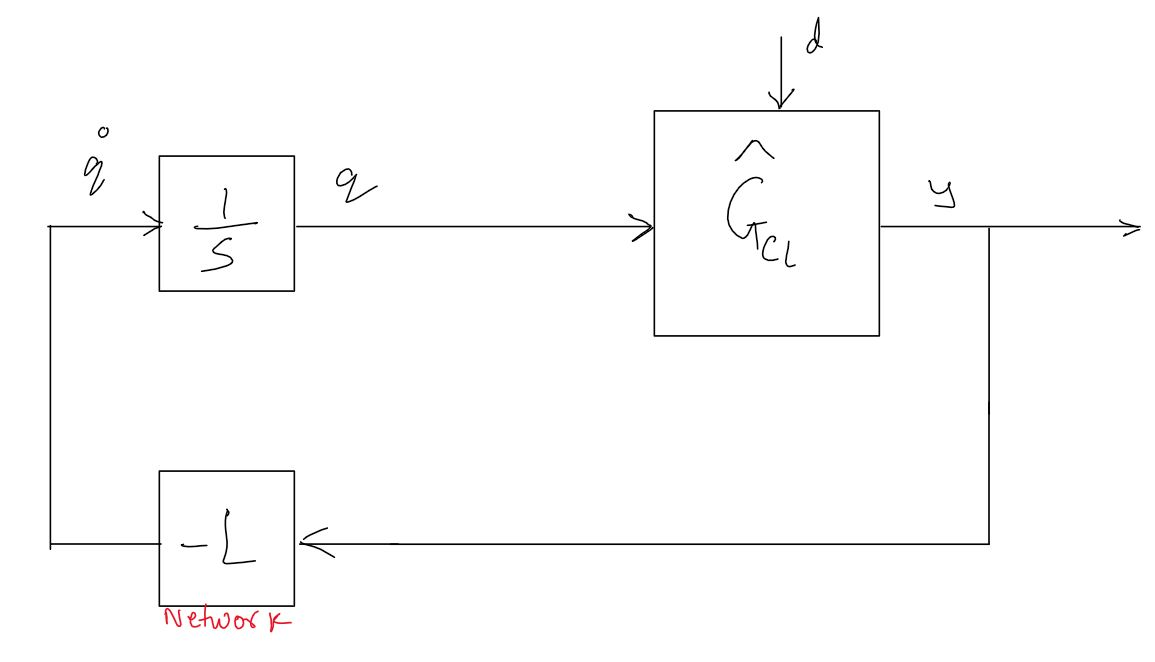
\includegraphics[height=0.45\textheight]{figures/cons_coupled.jpg}
	%\caption{Oil Spills}
	%\label{fig:oilspills}
\end{figure}
\begin{itemize}
	\item Can show stability (boundedness without assymptotic stability)
	\item Input output stability via a small-gain argument (Hespe's M. Thesis)
	\item Singular perturbation theory with a time-scale separation to prove assymptotic stability
\end{itemize}
\end{frame}
%%%%%%%%%%%%%%%%%%%%%%%%%%%%%%%%%%%%%%%%%%%%%%%%%%%%%%%%%%%%%%%%%%%%%
\begin{frame}{Flocking with a Coupled architecture}
	
\begin{figure}
	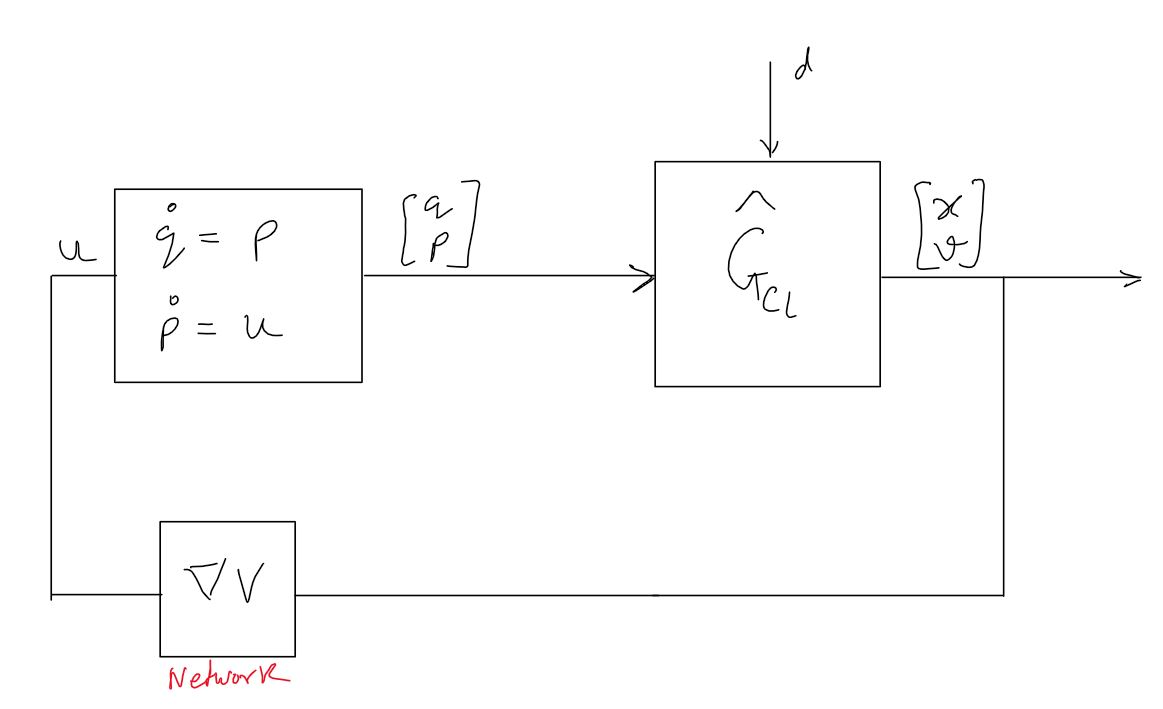
\includegraphics[height=0.45\textheight]{figures/Flocking_coupled.jpg}
	%\caption{Oil Spills}
	%\label{fig:oilspills}
\end{figure}
\begin{itemize}
	\item Attallah, Aly and Datar, Adwait and Werner, Herbert (2020): Flocking of Linear Parameter Varying Agents: Source Seeking Application with Underwater Vehicles. In 21st IFAC World Congress
	\item \textcolor{red}{No assymptotic stability yet}
\end{itemize}
\end{frame}
%%%%%%%%%%%%%%%%%%%%%%%%%%%%%%%%%%%%%%%%%%%%%%%%%%%%%%%%%%%%%%%%%%%%%
\begin{frame}{A more heuristic and practical architecture}
	
\begin{figure}
	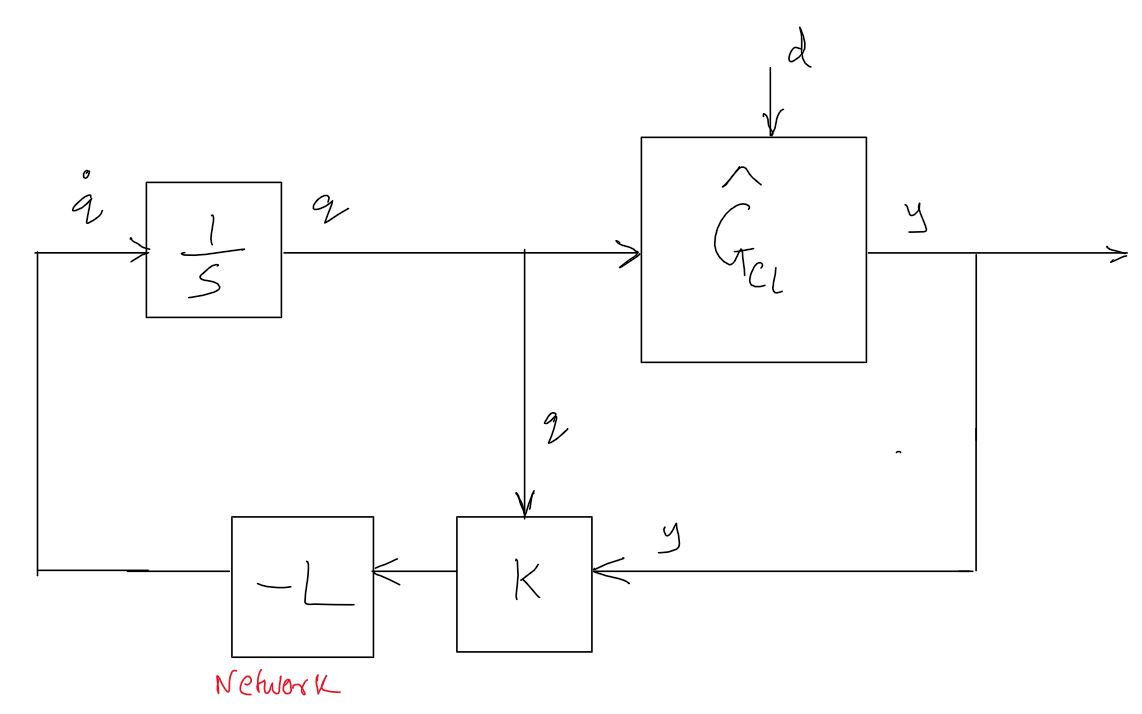
\includegraphics[height=0.45\textheight]{figures/cons_combined.jpg}
	%\caption{Oil Spills}
	%\label{fig:oilspills}
\end{figure}
\begin{itemize}
	\item Heuristic: Works well in Simulation
	\item \textcolor{red}{No analysis yet}
\end{itemize}
\end{frame}
%%%%%%%%%%%%%%%%%%%%%%%%%%%%%%%%%%%%%%%%%%%%%%%%%%%%%%%%%%%%%%%%%%%%%
\begin{frame}{Another commonly observed architecture}
	
	\begin{figure}
		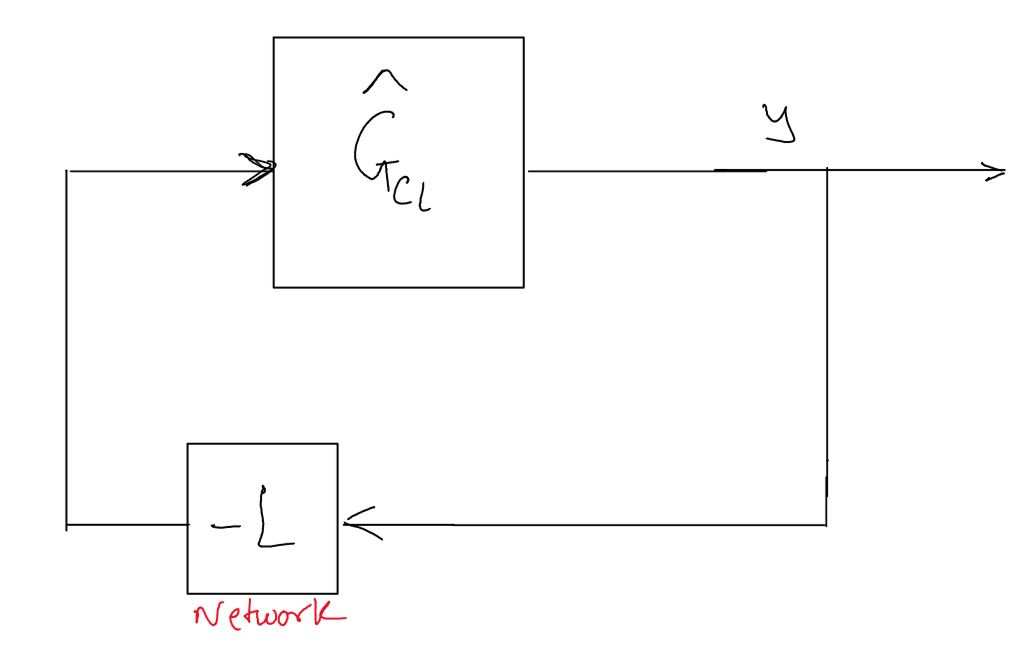
\includegraphics[height=0.45\textheight]{figures/general_arch_literture.jpg}
		%\caption{Oil Spills}
		%\label{fig:oilspills}
	\end{figure}
	\begin{itemize}
		\item Lot of literature on Stability Analysis for LTI systems
		\item Some of our past literature on Stability Analysis for LPV systems
		\item Some recent work on Passivity based analysis by Mark Spong and others
	\end{itemize}
\end{frame}
%%%%%%%%%%%%%%%%%%%%%%%%%%%%%%%%%%%%%%%%%%%%%%%%%%%%%%%%%%%%%%%%%%%%%
\begin{frame}{}
\begin{center}
    \huge{Thank you}
\end{center}
\end{frame}
%%%%%%%%%%%%%%%%%%%%%%%%%%%%%%%%%%%%%%%%%%%%%%%%%%%%%%%%%%%%%%%%%%%%%

\end{document}
